% !TEX root = ../main.tex
\chapter{KẾT QUẢ VÀ THẢO LUẬN}
\label{chap:results}

Chương này báo cáo các kết quả đã thu được theo thứ tự thực hiện ở Mục~\ref{sec:training-setup}:
\begin{itemize}
  \item chất lượng của các nguồn thông tin ý định;
  \item kết quả huấn luyện cặp mô hình B và D (bộ dữ liệu phản hồi sớm, nguồn hindsight);
  \item kiểm tra ngoại tuyến xem D có dùng thông tin ý định hay không;
  \item đánh giá vòng kín của B, D và expert.
\end{itemize}

Tại thời điểm viết, các mô hình A, C và các biến thể D với nguồn perfect, predicted chưa được huấn luyện. Vì vậy các câu hỏi Q1, Q2, Q4 và câu hỏi về nguồn thông tin mới được trả lời một phần (Mục~\ref{sec:results-status}). Mọi con số trong chương đều lấy trực tiếp từ các tệp kết quả của quy trình đánh giá. Không có số liệu nào được ước lượng hay điền tay.

\section{Chất lượng của các nguồn thông tin ý định}
\label{sec:source-quality}

\paragraph{Tia chỉ tay.} Trên 11\,391 khung chỉ tay của bộ dữ liệu phản hồi khi rõ, góc lệch giữa tia chỉ (gốc ngón trỏ $\to$ đầu ngón trỏ) và hướng tới tâm mục tiêu như sau:
\begin{itemize}
  \item trung bình $1{,}23^\circ$, độ lệch chuẩn $1{,}36^\circ$;
  \item phân vị 95\% là $4{,}61^\circ$, lớn nhất $6{,}22^\circ$.
\end{itemize}
Giá trị phân vị 95\% được dùng làm độ rộng $\sigma$ trong \eqref{eq:point}. Vì hai ô S bất kỳ cách nhau ít nhất $5^\circ$ theo hướng chỉ (Mục~\ref{sec:layout}), một tia chỉ lý tưởng gần như luôn phân biệt được mục tiêu. Độ khó của nguồn perfect vì vậy nằm chủ yếu ở \emph{thời điểm} chứ không ở hình học.

\paragraph{Cờ giữ vật.} Cờ ``đang giữ vật'' của bộ nhớ mục tiêu được suy ra từ độ mở kẹp. So với trạng thái gắp thật của mô phỏng, cờ này đạt:
\begin{itemize}
  \item precision 0,970, recall 0,988 (F1 0,979);
  \item độ trễ trung bình 0,68 khung khi gắp và 2,57 khung khi nhả (ở 20~Hz).
\end{itemize}
Bộ nhớ vì vậy không cần đọc trạng thái đặc quyền của mô phỏng để biết bước gắp đã hoàn thành.

\paragraph{Mức độ khớp giữa các nguồn.} Bảng~\ref{tab:source-agreement} cho tỉ lệ khung mà argmax của nguồn nhân quả trùng với nguồn hindsight trên bộ dữ liệu phản hồi sớm. Bảng tách theo vị trí của khung so với các mốc của cử chỉ. Có hai quan sát:
\begin{itemize}
  \item Sau $t_\text{clear}$ và ngoài các đoạn cử chỉ, cả hai nguồn nhân quả gần như trùng hoàn toàn với hindsight ($\geq 0{,}95$ ở hầu hết các trường).
  \item Khác biệt tập trung ở khoảng $[t_\text{onset}, t_\text{clear})$, đúng giai đoạn mà thông tin ý định được kỳ vọng có ích nhất. Tại đây \texttt{p\_target} của nguồn perfect chỉ trùng ở 61\% số khung, vì nguồn nhân quả cần thời gian tích lũy bằng chứng trước khi tin vào một mục tiêu.
\end{itemize}

Nguồn predicted ở bảng này dùng nhiễu bằng 0 (tham số nhiễu chưa được đo từ người thật), nên khác nguồn perfect chủ yếu ở bộ phân loại cử chỉ học được. Kết quả này vì vậy được đánh dấu là \emph{chưa hiệu chỉnh}.

\begin{table}[htbp]
  \centering
  \caption{Tỉ lệ khung có argmax trùng với nguồn hindsight (bộ dữ liệu phản hồi sớm). ``pp'': nguồn perfect; ``pr0'': nguồn predicted với nhiễu bằng 0 (chưa hiệu chỉnh).}
  \label{tab:source-agreement}
  \begin{tabular}{@{}llcccc@{}}
    \toprule
    \textbf{Nguồn} & \textbf{Trường} & $[t_\text{onset}, t_\text{clear})$ & $[t_\text{clear}, t_\text{end}]$ & \textbf{ngoài đoạn} & \textbf{tất cả} \\
    \midrule
    pp  & \texttt{p\_target} & 0,608 & 0,972 & 0,983 & 0,908 \\
        & \texttt{p\_who}    & 0,856 & 1,000 & 1,000 & 0,974 \\
        & \texttt{c\_target} & 0,838 & 1,000 & 0,999 & 0,970 \\
    \addlinespace
    pr0 & \texttt{p\_target} & 0,765 & 0,798 & 0,954 & 0,843 \\
        & \texttt{p\_who}    & 0,970 & 0,997 & 0,963 & 0,981 \\
        & \texttt{c\_target} & 0,914 & 1,000 & 0,999 & 0,984 \\
    \bottomrule
  \end{tabular}
\end{table}

\section{Kết quả huấn luyện}
\label{sec:training-results}

Hai mô hình B và D được huấn luyện 20\,000 bước trên bộ dữ liệu phản hồi sớm (Bảng~\ref{tab:train-results}). Trên tập kiểm định, hai mô hình gần như không khác nhau:
\begin{itemize}
  \item mất mát kiểm định: 0,259 với B và 0,261 với D;
  \item độ chính xác trên toàn đoạn 16 bước: D nhỉnh hơn B (0,916 so với 0,906);
  \item độ chính xác ở bước đầu tiên của đoạn, tức hành động thực sự được thực thi: B nhỉnh hơn (0,945 so với 0,936).
\end{itemize}
Mất mát huấn luyện của D thấp hơn rõ rệt (0,109 so với 0,136), trong khi mất mát kiểm định không giảm theo. Điều này gợi ý rằng thông tin ý định giúp D \emph{khớp tập huấn luyện} tốt hơn nhưng chưa giúp nó \emph{tổng quát hóa}.

\begin{table}[htbp]
  \centering
  \caption{Kết quả huấn luyện tại bước 20\,000 (bộ dữ liệu phản hồi sớm, nguồn hindsight cho D).}
  \label{tab:train-results}
  \begin{tabular}{@{}lcccc@{}}
    \toprule
    \textbf{Mô hình} & \makecell{Mất mát\\huấn luyện} & \makecell{Mất mát\\kiểm định} & \makecell{Độ chính xác\\kiểm định (đoạn)} & \makecell{Độ chính xác\\kiểm định (bước đầu)} \\
    \midrule
    B (không ý định) & 0,136 & 0,259 & 0,906 & 0,945 \\
    D (có ý định)    & 0,109 & 0,261 & 0,916 & 0,936 \\
    \bottomrule
  \end{tabular}
\end{table}

\section{Kiểm tra ngoại tuyến: D có dùng thông tin ý định không?}
\label{sec:offline-results}

Kiểm tra ngoại tuyến được chạy trên 27 episode kiểm định, trên mọi khung.

\paragraph{Độ chính xác hành động.} Bảng~\ref{tab:offline-accuracy} so sánh độ chính xác so với hành động của expert. Có ba quan sát:
\begin{itemize}
  \item D đạt 0,935 so với 0,923 của B. Lợi ích tập trung ở T2 (trao vật, $+3{,}1$ điểm phần trăm), T4 (xâm nhập, $+2{,}4$) và T5 (đổi ý, $+1{,}5$). Ở T1 và T3, hai mô hình gần như bằng nhau.
  \item Khi loại bỏ toàn bộ thông tin ý định, độ chính xác của D giảm về đúng mức của B (0,923), và hành động của D trùng với B ở 93,6\% số khung. Điều này phù hợp với mục đích của dropout toàn bộ: mô hình con ``không ý định'' xấp xỉ mô hình gốc.
  \item Tỉ lệ khởi động sớm sai bằng 0 với cả B, D và expert, chỉ tăng nhẹ lên 1,5\% khi D mất toàn bộ thông tin ý định.
\end{itemize}
Do tỉ lệ nhãn \texttt{HOLD} trong bộ dữ liệu này chỉ là 28,6\%, độ chính xác trên 0,9 không đến từ việc dự đoán toàn \texttt{HOLD}.

\begin{table}[htbp]
  \centering
  \caption{Độ chính xác hành động ngoại tuyến so với expert trên 27 episode kiểm định.}
  \label{tab:offline-accuracy}
  \begin{tabular}{@{}lccccccc@{}}
    \toprule
    \textbf{Mô hình} & \textbf{T1} & \textbf{T2} & \textbf{T3} & \textbf{T4} & \textbf{T4-neg} & \textbf{T5} & \textbf{Tất cả} \\
    \midrule
    B                       & 0,947 & 0,910 & 0,954 & 0,931 & 0,933 & 0,883 & 0,923 \\
    D                       & 0,946 & 0,941 & 0,954 & 0,955 & 0,933 & 0,898 & 0,935 \\
    D, bỏ toàn bộ ý định    & 0,944 & 0,902 & 0,949 & 0,942 & 0,933 & 0,887 & 0,923 \\
    \bottomrule
  \end{tabular}
\end{table}

\paragraph{Can thiệp phản thực tế.} Kết quả quan trọng nhất của kiểm tra ngoại tuyến nằm ở Bảng~\ref{tab:icr}: \textbf{D gần như không phản ứng với thông tin ý định}.
\begin{itemize}
  \item \textbf{Không gian.} Hoán đổi mục tiêu sang một ô hợp lệ khác cho $\text{ICR} = 0$ ở mọi khoảng trước $t_\text{clear}$, và chỉ 0,24\% sau đó. Tức là đổi vật mục tiêu trong thông tin ý định hầu như không làm D đổi hành động.
  \item \textbf{Ngữ nghĩa.} Hoán đổi vai trò cũng cho ICR dưới 0,2\%.
  \item \textbf{Thời gian và chuyển động.} Các nhóm này có ảnh hưởng lớn hơn: hoán đổi thời gian cho ICR 2,8\% trước $t_\text{clear}$; loại bỏ nhóm thời gian hoặc chuyển động cho ICR khoảng 2\%--2,7\%; loại bỏ toàn bộ cho 5,2\%.
\end{itemize}
Tiêu chí đặt trước ở Mục~\ref{sec:offline-checks} ($\text{ICR} \geq 0{,}3$ và $\text{CGR} \geq 0{,}6$ trước $t_\text{clear}$) \textbf{không đạt}. Hình~\ref{fig:actions-ep9} minh họa trên một episode T1: đường hành động của D gốc, D khi hoán đổi mục tiêu, D khi hoán đổi vai trò, D khi bỏ toàn bộ ý định và B gần như chồng khít lên nhau.

\begin{table}[htbp]
  \centering
  \caption{Tỉ lệ khung có hành động thay đổi (ICR) khi can thiệp vào thông tin ý định của D, trước và sau $t_\text{clear}$.}
  \label{tab:icr}
  \begin{tabular}{@{}llcc@{}}
    \toprule
    \textbf{Can thiệp} & \textbf{Nhóm} & \textbf{Trước $t_\text{clear}$} & \textbf{Sau $t_\text{clear}$} \\
    \midrule
    Hoán đổi & không gian & 0,0000 & 0,0024 \\
             & ngữ nghĩa  & 0,0014 & 0,0012 \\
             & thời gian  & 0,0278 & 0,0327 \\
    \addlinespace
    Loại bỏ  & ngữ nghĩa  & 0,0000 & 0,0009 \\
             & không gian & 0,0017 & 0,0009 \\
             & bộ nhớ     & 0,0006 & 0,0000 \\
             & thời gian  & 0,0199 & 0,0118 \\
             & chuyển động & 0,0267 & 0,0182 \\
             & toàn bộ    & 0,0523 & 0,0218 \\
    \bottomrule
  \end{tabular}
\end{table}

\begin{figure}[htbp]
  \centering
  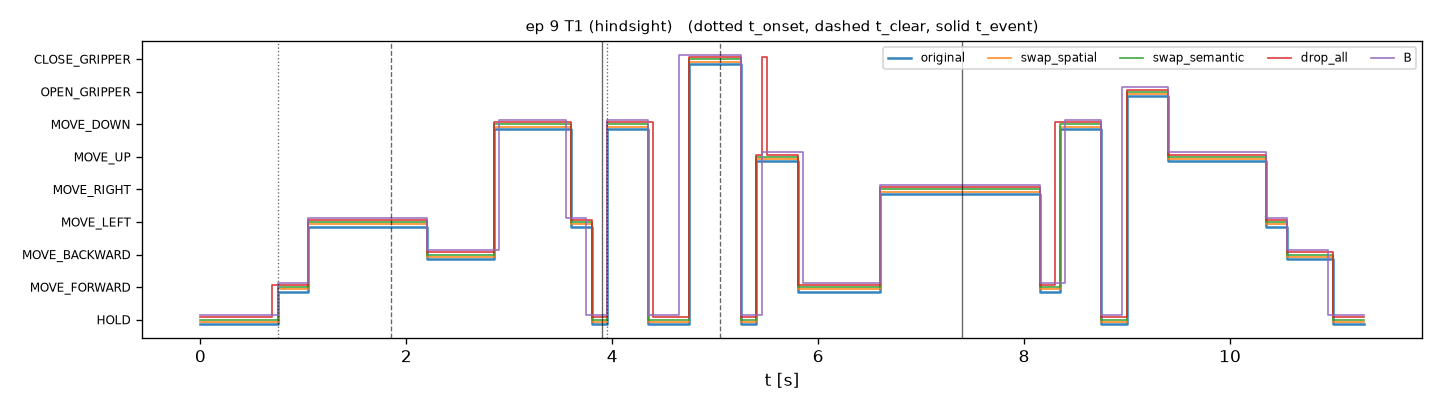
\includegraphics[width=\textwidth]{actions_ep9_T1}
  \caption{Hành động theo thời gian của D trên một episode T1 (episode 9) ở các chế độ: gốc, hoán đổi không gian, hoán đổi ngữ nghĩa, bỏ toàn bộ ý định, và mô hình B. Các vạch dọc là $t_\text{onset}$ (chấm), $t_\text{clear}$ (gạch) và $t_\text{event}$ (liền) của hai cử chỉ chỉ tay.}
  \label{fig:actions-ep9}
\end{figure}

\paragraph{Kiểm chứng quy tắc CGR.} Để tính CGR mà không phải mô phỏng lại mọi khung, khóa luận dùng một quy tắc xấp xỉ: hành động đúng là hành động đưa điểm công cụ về phía mục tiêu mới. Quy tắc này được đối chiếu với expert mô phỏng lại trên 25 khung và khớp ở 19 khung (76\%). Cả 6 khung không khớp đều rơi vào giai đoạn expert mở kẹp trong T3, nơi quy tắc ``đi về phía mục tiêu'' không mô tả đúng hành động mở kẹp. Vì CGR chỉ có ý nghĩa khi ICR đủ lớn, hạn chế này chưa ảnh hưởng tới kết luận ở trên.

\section{Đánh giá vòng kín}
\label{sec:closed-loop-results}

Bảng~\ref{tab:closed-loop} cho tỉ lệ hoàn thành nhiệm vụ trên 120 episode đánh giá.

\paragraph{Expert.} Expert phản hồi sớm đạt CSR 0,892, với các lỗi như sau:
\begin{itemize}
  \item hết thời gian ở T2 và T4;
  \item làm đổ cốc ở T3;
  \item dừng không cần thiết ở T4-neg.
\end{itemize}
Đây là mức tham chiếu của dữ liệu trình diễn.

\paragraph{Hai chính sách học được.} Cả hai đều \textbf{thất bại gần như hoàn toàn}:
\begin{itemize}
  \item B hoàn thành 1/120 episode (CSR 0,008);
  \item D hoàn thành 11/120 episode (CSR 0,092);
  \item gần như mọi thất bại đều do \emph{hết thời gian}.
\end{itemize}
Tỉ lệ thời gian robot đứng yên (IR) cho thấy nguyên nhân: ở vai Instructor, IR là 0,999 với B và 0,918 với D, so với 0,000 của expert. Nghĩa là chính sách gần như đứng yên suốt episode thay vì làm sai.

\paragraph{An toàn.} Về an toàn, cả ba đều không có va chạm (CFR $= 1$). HCS của B (0,979) và D (1,000) cao hơn expert (0,926). Tuy nhiên kết quả này chủ yếu phản ánh việc robot ít chuyển động, không phải chính sách an toàn hơn.

\begin{table}[htbp]
  \centering
  \caption{Tỉ lệ hoàn thành nhiệm vụ (CSR) trong đánh giá vòng kín, 20 episode mỗi nhiệm vụ.}
  \label{tab:closed-loop}
  \begin{tabular}{@{}lccccccc@{}}
    \toprule
    \textbf{Tác tử} & \textbf{T1} & \textbf{T2} & \textbf{T3} & \textbf{T4} & \textbf{T4-neg} & \textbf{T5} & \textbf{Tất cả} \\
    \midrule
    Expert (phản hồi sớm) & 1,00 & 0,85 & 0,85 & 0,85 & 0,85 & 0,95 & 0,892 \\
    B                     & 0,00 & 0,00 & 0,05 & 0,00 & 0,00 & 0,00 & 0,008 \\
    D                     & 0,05 & 0,15 & 0,00 & 0,15 & 0,15 & 0,05 & 0,092 \\
    \bottomrule
  \end{tabular}
\end{table}

\section{Thảo luận}
\label{sec:discussion}

\paragraph{Khoảng cách giữa ngoại tuyến và vòng kín.} Độ chính xác từng bước trên 0,92 nhưng tỉ lệ hoàn thành dưới 0,1 là biểu hiện điển hình của lỗi tích lũy do lệch phân phối~\cite{ross2011dagger}. Trong một episode dài vài trăm bước, chỉ cần chính sách rơi vào một trạng thái mà nó dự đoán \texttt{HOLD}, robot sẽ đứng yên. Trạng thái của robot khi đó không đổi, ảnh camera gần như không đổi, nên quyết định tiếp theo cũng không đổi. Chỉ số IR gần 1 ủng hộ cách giải thích này.

Ngoài ra, dữ liệu trình diễn chứa nhiều giai đoạn mà robot \emph{phải} đứng chờ người, ví dụ khi chờ người ra hiệu xong hay chờ người cầm vật. Những trạng thái chờ này có thể trông rất giống các trạng thái robot cần di chuyển. Vì chính sách không có bộ nhớ và chỉ thực thi một bước mỗi lần, nó khó phân biệt hai loại trạng thái. Hai hướng khắc phục tự nhiên là:
\begin{itemize}
  \item thu thêm dữ liệu có nhiễu theo DART~\cite{laskey2017dart}, hoặc sửa nhãn trên chính trạng thái của chính sách theo DAgger~\cite{ross2011dagger};
  \item kiểm tra lại sự nhất quán giữa đường ống quan sát lúc huấn luyện và lúc chạy vòng kín.
\end{itemize}

\paragraph{Vì sao D bỏ qua thông tin không gian.} Kết quả kiểm tra ngoại tuyến cho thấy D dựa vào nhóm thời gian và chuyển động nhiều hơn nhóm không gian. Một giải thích hợp lý nằm ở chính dữ liệu trình diễn. Expert phản hồi sớm chỉ cam kết với mục tiêu sau khi bằng chứng đã xuất hiện, ở 40\% chuyển động tiết lộ ý định. Tại thời điểm đó, tay người đã hướng rõ về mục tiêu trong ảnh camera \texttt{high}. Như vậy, trong dữ liệu huấn luyện, mục tiêu luôn \emph{nhìn thấy được} từ ảnh vào đúng lúc nó cần cho hành động. Thông tin ý định không gian vì vậy dư thừa so với ảnh, và mạng không có động lực để đọc nó.

Ngược lại, thông tin thời gian (cử chỉ đã đi được bao nhiêu, còn bao lâu nữa) khó đọc từ một ảnh tĩnh, nên được dùng nhiều hơn. Điều này cũng giải thích vì sao lợi ích ngoại tuyến của D tập trung ở T2 và T4, hai nhiệm vụ mà thời điểm quyết định thành bại.

Quan sát này có hệ quả quan trọng cho thiết kế thí nghiệm: \emph{thông tin ý định chỉ có thể giúp khi dữ liệu trình diễn đòi hỏi hành động trước khi ảnh đủ để suy ra mục tiêu}. Các hướng xử lý tiếp theo gồm:
\begin{itemize}
  \item bỏ thời gian chờ 1,6~s trước khi gắp trong chế độ phản hồi sớm, để robot hành động ngay khi có thông tin;
  \item che hoặc làm nhiễu vùng người trong ảnh khi huấn luyện, buộc mạng dùng thông tin ý định;
  \item bật nhánh FiLM để thông tin ý định tác động trực tiếp lên đặc trưng ảnh;
  \item huấn luyện lâu hơn (50\,000 bước).
\end{itemize}

\paragraph{Về câu hỏi Q3.} Với dữ liệu hiện có, câu trả lời cho Q3 là \emph{chưa}: trên dữ liệu phản hồi sớm, D chỉ nhỉnh hơn B 1,2 điểm phần trăm về độ chính xác ngoại tuyến, và không vượt qua kiểm tra ``có dùng thông tin ý định''. D đạt CSR vòng kín cao hơn B (0,092 so với 0,008), nhưng cả hai đều quá xa expert để có thể kết luận về lợi ích của thông tin ý định.

\section{Các kết quả còn chờ}
\label{sec:results-status}

Bảng~\ref{tab:pending} tổng hợp trạng thái của các thí nghiệm.

\begin{table}[htbp]
  \centering
  \caption{Trạng thái các thí nghiệm tại thời điểm viết.}
  \label{tab:pending}
  \small
  \begin{tabularx}{\textwidth}{@{}l l X@{}}
    \toprule
    \textbf{Thí nghiệm} & \textbf{Trạng thái} & \textbf{Ghi chú} \\
    \midrule
    B, D (hindsight)   & đã có & Mục~\ref{sec:training-results}--\ref{sec:closed-loop-results} \\
    A, C               & chưa chạy & dữ liệu phản hồi khi rõ đã thu (274 episode) \\
    D (perfect)        & chưa chạy & nguồn đã cài đặt, đã đo mức khớp (Bảng~\ref{tab:source-agreement}) \\
    D (predicted)      & chưa chạy & cần đo tham số nhiễu từ người thật \\
    Giữ lại theo nhóm  & một phần & mới có loại bỏ từng nhóm (Bảng~\ref{tab:icr}) \\
    \bottomrule
  \end{tabularx}
\end{table}

\todo{Cập nhật chương này khi có kết quả A, C và các nguồn perfect, predicted.}
